In der Theorie gab es so viele Filialen wie Schülerteams, welche ebenfalls untereinander vernetzt werden sollten. Hierfür wurde wie \ref{fig:netzplan_gesamt} zu entnehmen ist, das gegebene Netz in
16 Subnetze unterteilt und neun davon auch tatsächlich benutzt. Diese Subnetze wurden dann pro Team erneut unterteilt um die Abteilungen entsprechend darzustellen \ref{fig:subnetze}. 

\begin{figure}[h]
	\centering
	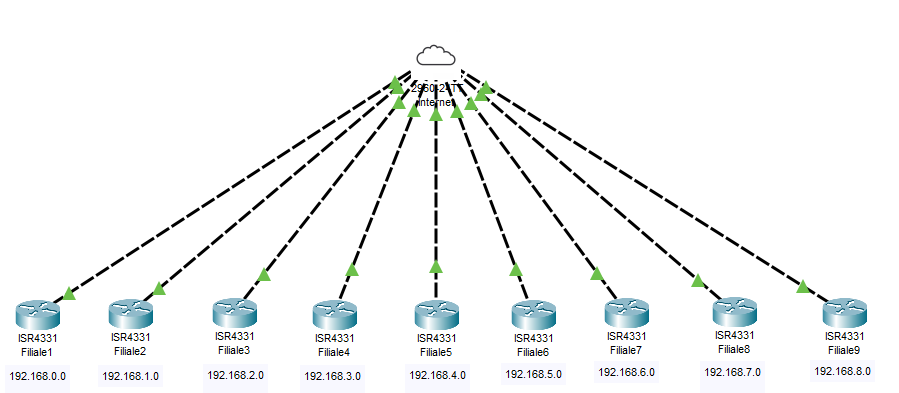
\includegraphics[width=15cm]{images/Netzplan_gesamt.png}
	\caption[Netzplan gesamt]{Darstellung aller verwendeten Subnetze der Filialen}
	\label{fig:netzplan_gesamt}
\end{figure}

Die theoretische Verkabelung unterscheidet sich im Wesentlichen davon vom praktischen Aufbau, dass hier alle Abteilungen und alle Endgeräte berücksichtigt wurden und sich somit
mehr Geräte im Netz befinden und entsprechend auch eine größere Anzahl an Geräten konfiguriert werden muss. In der theoretischen Netzwerkplanung wurde der Access-Point jedoch noch nicht 
berücksichtigt. Der theoretische Aufbau mit allen Netzwerk- und Endgeräten, wie er in einer Filiale vorliegen würde, wird in \ref{fig:netzplan_filiale} dargestellt.

\begin{figure}[h]
	\centering
	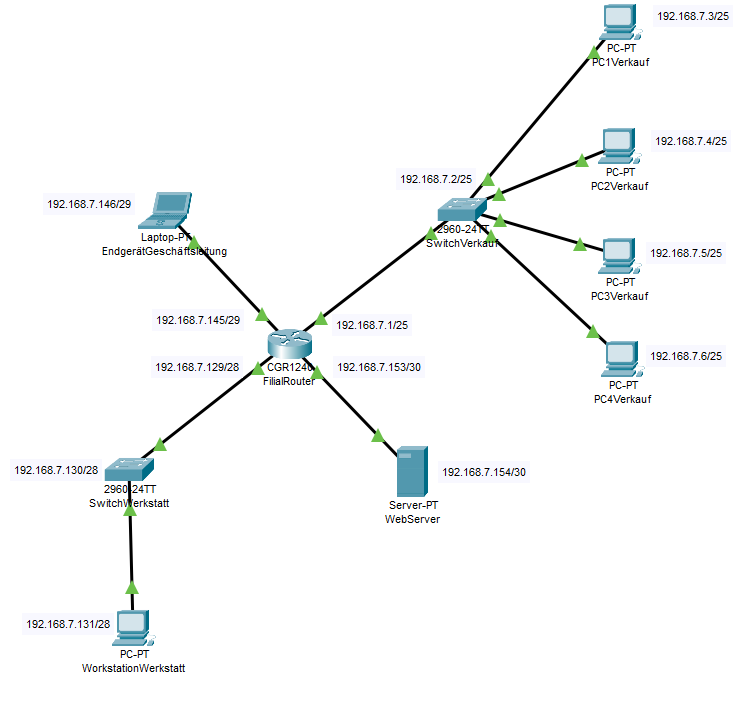
\includegraphics[width=15cm]{images/Netzplan_Filiale.png}
	\caption[Netzplan Filiale]{Darstellung der Subnetze und Geräte in der Filiale}
	\label{fig:netzplan_filiale}
\end{figure}